\chapter{Implementasi dan Pengujian}
\label{chap:implementasipengujian}
Pada bab ini akan diimplementasikan kode program untuk propagasi email dan pengujian dua skenario yang ada pada Bab ~\ref{chap:analisis}.

\section{Lingkungan Implementasi}
\label{sec:lingkunganimplementasi}
Implementasi dilakukan pada lingkungan :
\begin{enumerate}
	\item Eclipse 4.5 Mars
	\item BPMN versi 2.0 dan Camunda Modeler versi 1.7.2.
	\item BPMS Camunda versi 7.6.0 dan berjalan pada tomcat versi 8.0.24.
	
\end{enumerate}
\section{Implementasi Kode Program}
\label{sec:kodeprogram}


\subsection{Implementasi Algoritma Pengiriman Email}
\label{implementasialgo}
Beberapa potongan kode di bawah ini adalah kode untuk pengiriman email. Kode secara keseluruhan dapat dilihat pada Lampiran~\ref{lamp:tasklistener}
\begin{itemize}
	\item Konfigurasi email admin.
\begin{lstlisting}[language=Java,basicstyle=\tiny,caption=TaskAssignmentListener.java]
  private static final String HOST = "smtp.gmail.com";
  private static final String USER = "camundasys@gmail.com";
  private static final String PWD = "epW3S4KN";
\end{lstlisting}
	

	\item Kode untuk mengambil assignee (aktor dari \textit{task}, mengambil id \textit{task}, dan mengambil alamat email aktor.
	\begin{lstlisting}[language=Java,basicstyle=\tiny,caption=TaskAssignmentListener.java]

 public void notify(DelegateTask delegateTask) {
    String assignee = delegateTask.getAssignee();
    String taskId = delegateTask.getId();
\end{lstlisting}

	\item Konfigurasi SMTP Gmail.
	\begin{lstlisting}[language=Java,basicstyle=\tiny,caption=TaskAssignmentListener.java]

               props = System.getProperties();
               props.put("mail.smtp.port", "587");
               props.put("mail.smtp.auth", "true");
               props.put("mail.smtp.starttls.enable", "true");

\end{lstlisting}
	\item Kode untuk mendapatkan aktor apabila atribut assignee memiliki nilai.
	\begin{lstlisting}[language=Java,basicstyle=\tiny,caption =TaskAssignmentListener.java]
	if (assignee != null) {
      IdentityService identityService = Context.getProcessEngineConfiguration().getIdentityService();
      User user = identityService.createUserQuery().userId(assignee).singleResult();
      if (user != null) {
    	  this.sendEmail(user);
      }
    }
	\end{lstlisting}
	
		\item Kode untuk mendapatkan aktor apabila atribut assignee tidak memiliki nilai.
	\begin{lstlisting}[language=Java,basicstyle=\tiny,caption =TaskAssignmentListener.java]
	    	TaskEntity task = (TaskEntity)delegateTask;
    	List<IdentityLinkEntity> identityLinks = task.getIdentityLinks();
    	
    	for(IdentityLinkEntity link : identityLinks) {
    		if(link.getType().equals(IdentityLinkType.CANDIDATE)) {
    		    if(link.isUser()) {
	    		     User user = Context.getProcessEngineConfiguration().getIdentityService().createUserQuery().userId(link.getUserId()).singleResult();
	    		     sendEmail(user);
    		    }
    		    if(link.isGroup()) {
    		        List<User> users = Context.getProcessEngineConfiguration().getIdentityService().createUserQuery().memberOfGroup(link.getGroupId()).list();
    		        for(User user : users) {
    		        	sendEmail(user);
    		        }
    		    }
    		}
    	}
	\end{lstlisting}
	
	

	\item Kode untuk membangkitkan subjek dan isi email
	\begin{lstlisting}[language=Java,basicstyle=\tiny,caption=TaskAssignmentListener.java]

 session = Session.getDefaultInstance(props, null);
               message = new MimeMessage(session);
               message.addRecipient(Message.RecipientType.TO, new InternetAddress(recipient));
               message.setSubject("Task " + delegateTask.getName());
               
               String emailBody = user.getFirstName() +",<br>";
          emailBody += "Tolong Selesaikan Task " +taskName + " di bawah ini.<br>";
          emailBody += "http://localhost:1234/camunda/app/tasklist/default/#/?task="+taskId;
          message.setContent(emailBody, "text/html");
\end{lstlisting}

	\item Kode untuk mengirimkan email.
	\begin{lstlisting}[language=Java,basicstyle=\tiny,caption=TaskAssignmentListener.java]

Transport transport = session.getTransport("smtp");            
               transport.connect(HOST, USER, PWD);
               transport.sendMessage(message, message.getAllRecipients());
               transport.close();
\end{lstlisting}
	
\end{itemize}

\subsection{Implementasi Skenario}
\label{implementasiskenario}

\subsubsection{Pengajuan Proposal Bisnis dan Pengajuan Proposal Bisnis dari Grup}
Kode ini adalah kode file HTML untuk Skenario~\ref{skenario1} dan Skenario~\ref{skenario2}. Terdapat dua form HTML yaitu MengunggahDokumen.html dan MemeriksaDokumen.html. 
\begin{lstlisting}[language=html,basicstyle=\tiny,caption=MengunggahDokumen.html]
<html>
<head>
<body>
	<form method="post" name="upload-dokumen">
		<input type="file"
       cam-variable-name="proposal"
       cam-variable-type="File"
       cam-max-filesize="10000000"/>
	</form>
</body>
</html>

\end{lstlisting}

\begin{lstlisting}[language=html,basicstyle=\tiny,caption=MemeriksaDokumen.html]


<html>
<head></head>

<body>
<form role="form" name="form">
  	<a cam-file-download="proposal">Download Dokumen</a>
    <p>Apakah Proposal layak?</p>
    <input cam-variable-name="valid"
             cam-variable-type="Boolean"
             type="checkbox"
             name="valid"
             class="form-control" />  
</form> 
</body>
</html>

\end{lstlisting}

\section{Pengujian}
\label{sec:pengujian}

\subsection{Pengujian Skenario 1}
label{ujiskenario1}
Pada Skenario ~\ref{skenario1}, ditambahkan form HTML dan Task Listener untuk mengirimkan email.
		\begin{figure}[H]
			\centering
			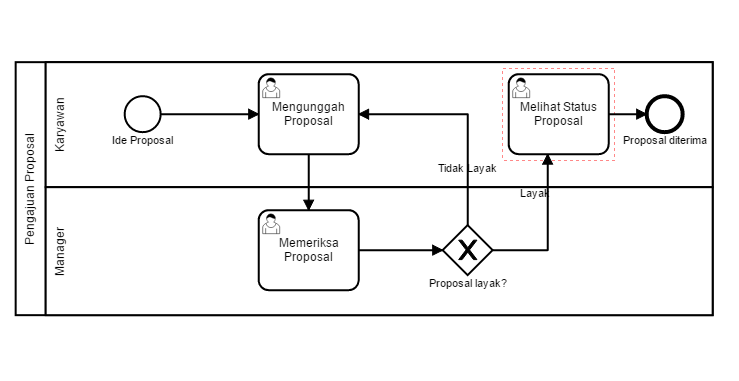
\includegraphics[scale=0.5]{Gambar/Bab-5/bpmn1}
			\caption{Mengunggah Proposal} 
			\label{fig:mengunggah proposal}
		\end{figure}
		
Proses pengujian :
\begin{itemize}
	\item John mengunggah dokumen proposal
				\begin{figure}[H]
			\centering
			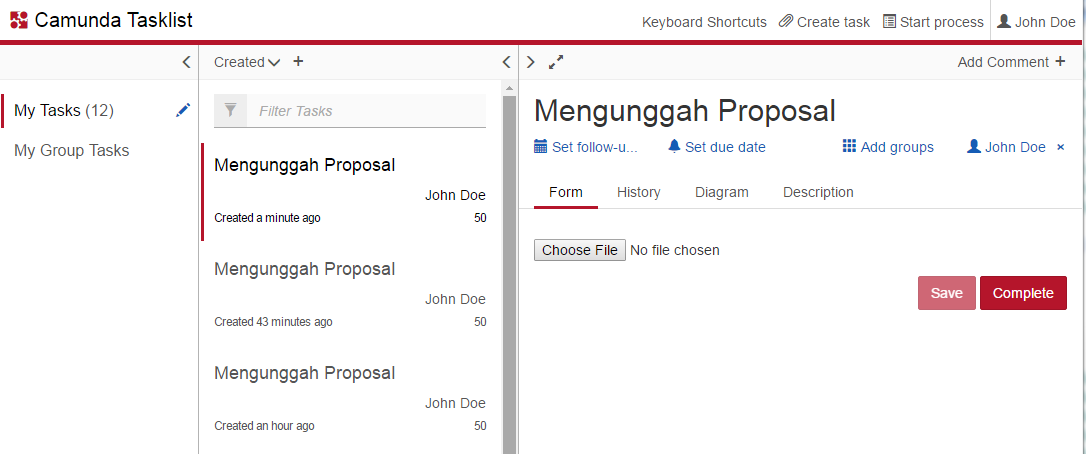
\includegraphics[scale=0.5]{Gambar/Bab-5/uji1-1}
			\caption{Mengunggah Proposal} 
			\label{fig:unggahProposal}
		\end{figure}
	\item Peter mendapatkan email dari sistem Camunda yang memberitahukan \textit{task} terbaru
	\begin{figure}[H]
			\centering
			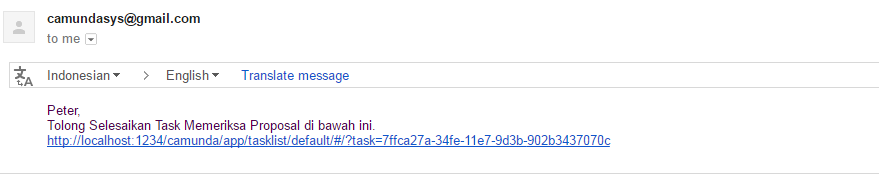
\includegraphics[scale=0.5]{Gambar/Bab-5/uji1-2}
			\caption{Menerima Email} 
			\label{fig:menerimaEmail}
		\end{figure}
	\item Tautan email membawa Peter ke \textit{task} yang harus dikerjakan.
		\begin{figure}[H]
			\centering
			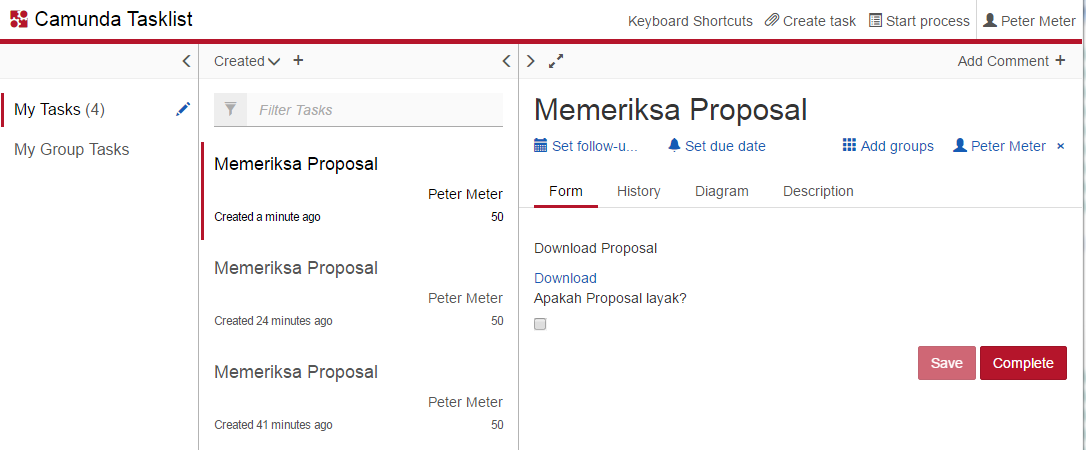
\includegraphics[scale=0.5]{Gambar/Bab-5/uji1-3}
			\caption{Tasklist Peter} 
			\label{fig:tasklistPeter}
		\end{figure}
	\end{itemize}
	
		
		
\subsection{Pengujian Skenario 2}
\label{ujiskenario2}
Pada Skenario ~\ref{skenario2}, ditambahkan form HTML dan Task Listener untuk mengirimkan email. Perbedaan dengan Skenario ~\ref{skenario1} adalah \textit{task} didelegasikan ke grup \textit{accounting}, \textit{sales}, dan \textit{management}. John adalah bagian dari divisi \textit{sales}, Mary adalah bagian dari divisi \textit{accounting}, sedangkan Peter adalah bagian dari divisi {\textit{management}.
		\begin{figure}[H]
			\centering
			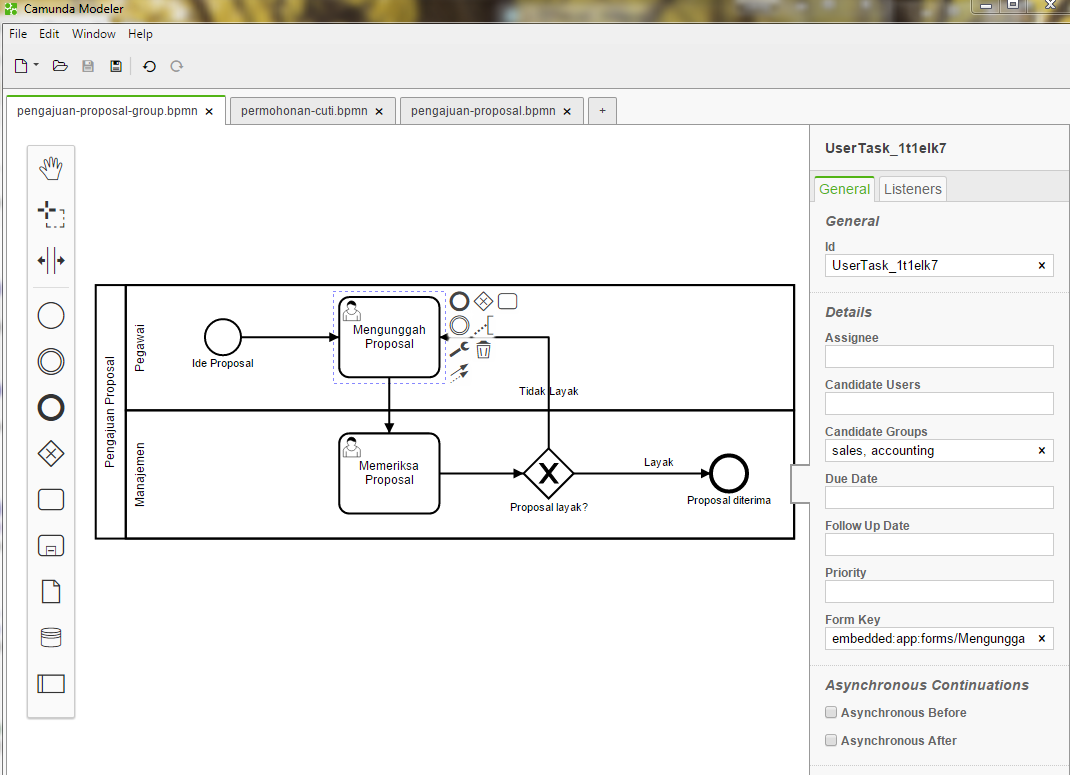
\includegraphics[scale=0.5]{Gambar/Bab-5/bpmn2}
			\caption{Mengunggah Proposal Group} 
			\label{fig:mengunggah proposal Group}
		\end{figure}
		
Proses pengujian :
\begin{itemize}
	\item Admin memulai proses
		\begin{figure}[H]
			\centering
			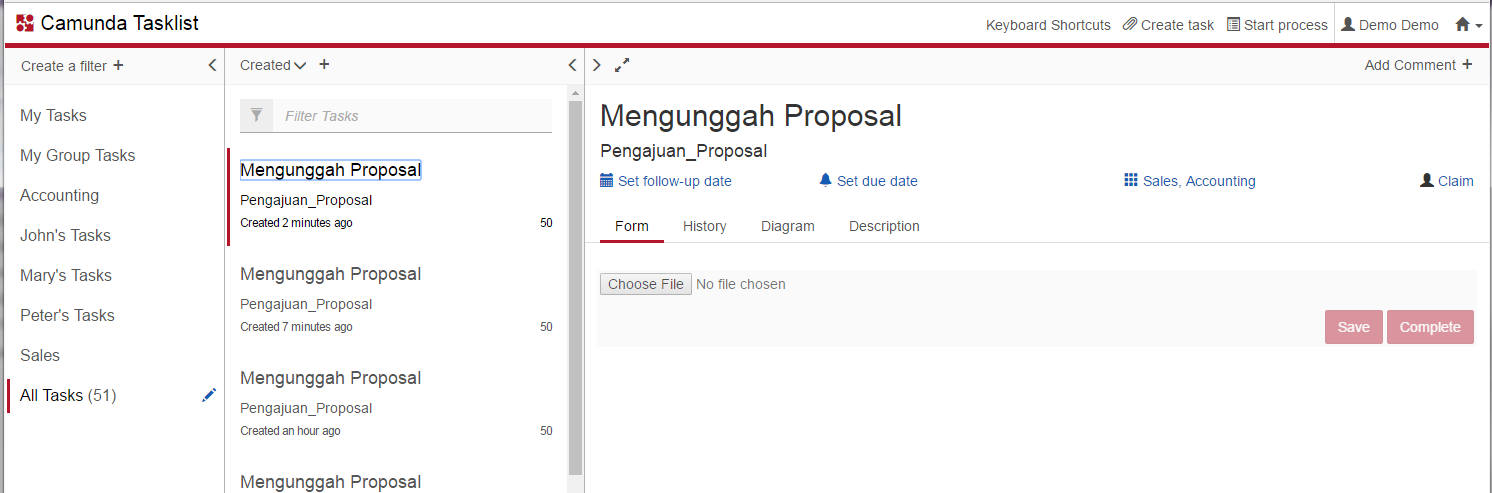
\includegraphics[scale=0.4]{Gambar/Bab-5/uji2-1}
			\caption{John Mengunggah Proposal} 
			\label{fig:johnUnggahProposal}
		\end{figure}

	\item John dan Mary mendapatkan email untuk mengerjakan \textit{task}.
		\begin{figure}[H]
			\centering
			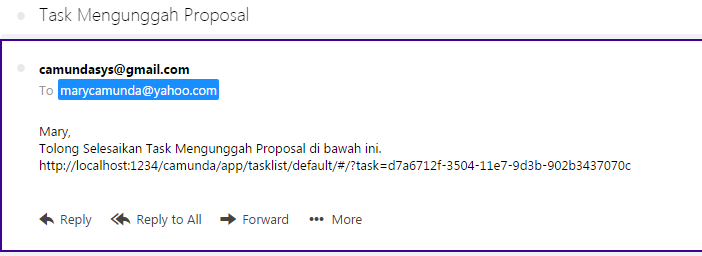
\includegraphics[scale=0.5]{Gambar/Bab-5/uji2-2}
			\caption{Mary Mendapat Email} 
			\label{fig:marydapatemail}
		\end{figure}
		
		\begin{figure}[H]
			\centering
			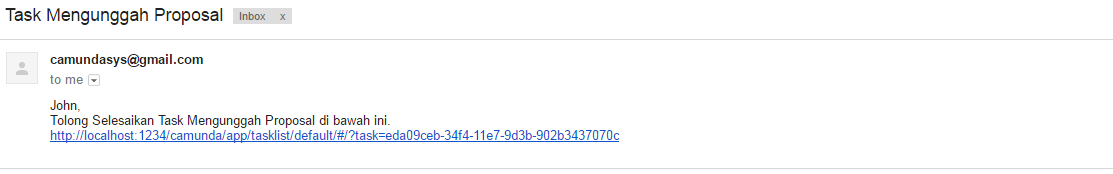
\includegraphics[scale=0.5]{Gambar/Bab-5/uji2-3}
			\caption{John Mendapat Email} 
			\label{fig:johndapatemail}
		\end{figure}

	\item John dan Mary dapat mengklaim \textit{task}. Apabila John mengklaim \textit{task}, maka Mary tidak bisa mengklaim \textit{task}.
			\begin{figure}[H]
			\centering
			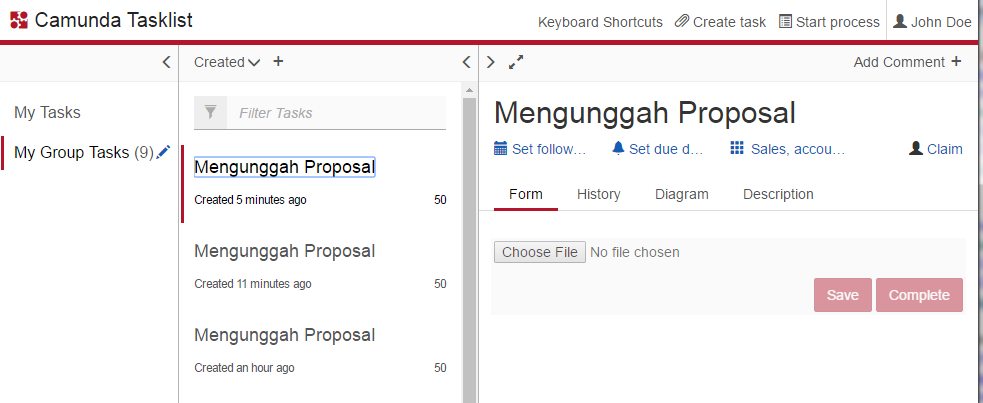
\includegraphics[scale=0.5]{Gambar/Bab-5/uji2-4}
			\caption{John Mengunggah Proposal} 
			\label{fig:johnUnggahProposal}
		\end{figure}
		
\begin{figure}[H]
			\centering
			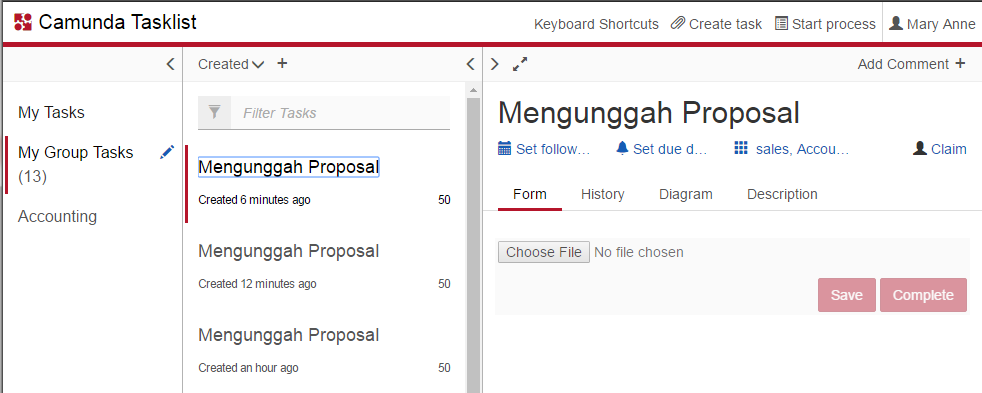
\includegraphics[scale=0.5]{Gambar/Bab-5/uji2-5}
			\caption{Mary Mengunggah Proposal} 
			\label{fig:maryUnggahProposal}
		\end{figure}
		
	\item Mary mengklaim task dan mengerjakan \textit{task}
		\begin{figure}[H]
			\centering
			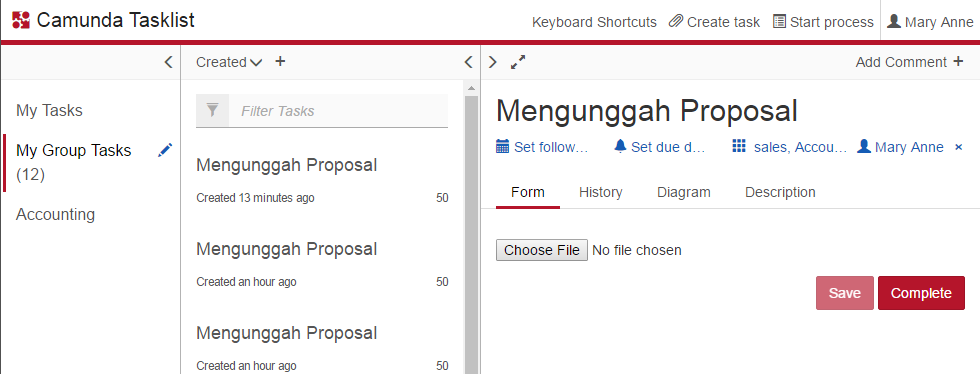
\includegraphics[scale=0.5]{Gambar/Bab-5/uji2-6}
			\caption{Mary mengklaim Task} 
			\label{fig:maryklaimtask}
		\end{figure}
	
	\item Peter mendapatkan email untuk mengerjakan \textit{task}.
		\begin{figure}[H]
			\centering
			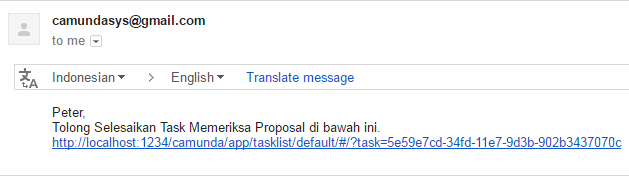
\includegraphics[scale=0.5]{Gambar/Bab-5/uji2-7}
			\caption{Mary mengklaim Task} 
			\label{fig:maryklaimtask}
		\end{figure}
		
	\item Peter mengklaim task dan menolak proposal
		\begin{figure}[H]
			\centering
			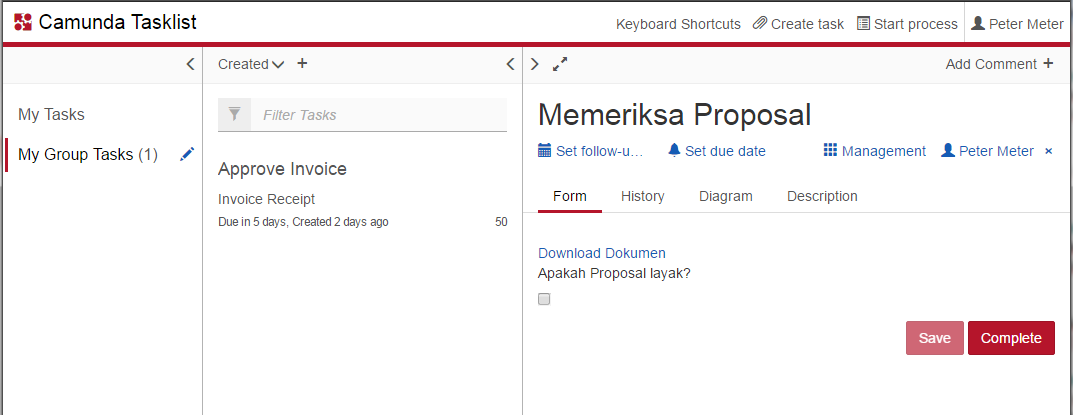
\includegraphics[scale=0.5]{Gambar/Bab-5/uji2-8}
			\caption{Peter mengklaim Task} 
			\label{fig:peterklaimtask}
		\end{figure}
	
	\item John dan Mary mendapatkan email sistem Camunda yang memberitahukan \textit{task} terbaru
		\begin{figure}[H]
			\centering
			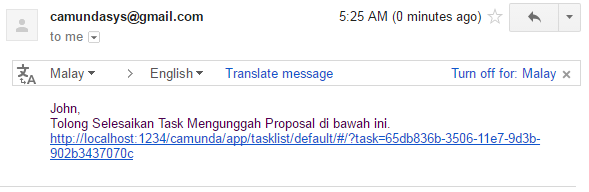
\includegraphics[scale=0.5]{Gambar/Bab-5/uji2-9}
			\caption{John mendapatkan Email} 
			\label{fig:johndapatemail}
		\end{figure}
	
	\begin{figure}[H]
			\centering
			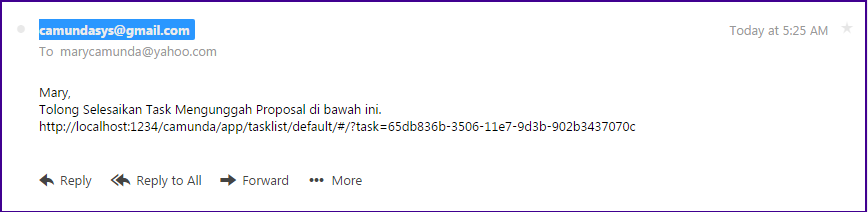
\includegraphics[scale=0.5]{Gambar/Bab-5/uji2-10}
			\caption{Mary mendapatkan Email} 
			\label{fig:marydapatemail}
		\end{figure}
\end{itemize}

\section{Hasil Pengujian}
Pengujian sudah berhasil untuk semua skenario. Pada skenario 1, John dan Peter masing-masing mendapatkan email ketika \textit{task} siap dikerjakan. Pada skenario 2, Setiap karyawan (John dan Mary) mendapatkan email untuk membuat proposal. Peter juga mendapat email setelah John atau Mary mengunggah proposal.